\documentclass[../../labo_tp5_main.tex]{subfiles}

\begin{document}

%capítulo
\section{Ejercicio 5}

El Ente Nacional de Comunicaciones (ENACOM) define al espectro radioel\'ectrico como "el conjunto de frecuencias que, conforme a la tecnología disponible, pueden ser empleadas para emitir ondas que permitan transportar información". Dado que es considerado un recurso natural sobre el cual el Estado tiene el control, se lo divide en bandas que son atribuidas a distintos Servicios y Sistemas de Comunicaciones Radioel\'ectricas. Esta atricuci\'on se muestra en la tabla \ref{tab:cabfra}.

\begin{table}[H]
\begin{tabular}{|l|L{6cm}|L{6cm}|}
\hline
SERVICIO            & FRECUENCIAS DE OPERACIÓN                                                                                                                                                           & POTENCIA IRRADIADA                                                                                                                                 \\
\hline
Radiodifusión de AM & 535 - 1705 kHz                                                                                                                                                                     & Mín 100 W Máx 100 kW                                                                                                                               
\\
\hline
Radiodifusión de FM & 88 - 108 MHz                                                                                                                                                                       & Mín 30 W Max 100 kW                                                                                                                                \\
\hline
Radiodifusión de TV & TV abierta \textbf{VHF bajo:} 54 - 72 MHz (canales 2-4) 76 - 88 MHz (c. 5-6) \textbf{VHF alto:} 174 - 216 MHz (c. 7-13) \textbf{UHF} (en gral. TV codificada, o sea no abierta)512 - 806 MHz (21-69) & \textbf{VHF:} Mín 5 kw en estación autónoma, 50 W en repetidora. Máx 30 kW en transmisor irradiado hasta 150 kW \textbf{UHF} (codificado, área reducida):aprox. 25 W \\
\hline
Telefonía celular   & \textbf{SRMC/STM:} 869 - 894 MHz (base) 824 - 849 MHz (móvil) \textbf{PCS:} 1850 - 1910 MHz (móvil)1930 - 1990 MHz (base)                                                                            & Celdas en zona muy urbanizada: Aprox. 20 WZona rural: máx. 100 W                                                                                   \\
\hline
HF                  & Servicio fijo y móvil (en gral uso comercial): 2 - 30 MHzRadioaficionados:bandas en los rangos de 1,8 - 3,6 - 3,8 - 7 -10 - 14 - 18 - 21 - 25 y 29 MHz                             & Se especifica potencia pico de envolvente (la potencia media está unos 10 dB por debajo) Uso comercial: máx 160 WRadioafición: máximo 1,5 kW       \\
\hline
VHF y UHF           & \textbf{{[}MHz{]}}30 - 50138 - 174242 - 280340 - 399421 - 426443 - 490                                                                                                                      & Handies 6 W Móvil 40 WBase 60 WEstos son valores típicos                                                                                           \\
\hline
Móvil Marítimo      & \textbf{Rangos HF:} 4, 6, 8, 12, 16, 18, 22, 25 MHz \textbf{Rangos VHF}: 156, 0 - 157,5 /160,5 - 162 MHz                                                                                             & \textbf{HF}: aprox. 150 W pico de envolvente \textbf{VHF}: 25 W                                                                                                      \\
\hline
Móvil Aeronáutico   & \textbf{HF (AM)}: entre 2 y 30 MHz \textbf{VHF:} 108 - 118 MHz radionavegación (ILS, VOR)118 - 136 MHz comunicaciones móvil - tierra                                                                 & \textbf{HF}: hasta 400 W PEP (media 100 W) \textbf{VHF}: 20 W\\
\hline
 
\end{tabular}

\caption{CABFRA (Cuadro de Atribuci\'on de Bandas de Frecuencias de la Rep\'ublica Argentina}
\label{tab:cabfra}
\end{table}

Con esto en mente, se intent\'o sintonizar una emisi\'on que no correspondiera a ninguna radio AM ni FM, ni televisi\'on. Si bien se lograron observar picos de potencia en el espectro (por ejemplo, el canal de emergencia de la banda VFH del Servicio M\'ovil Mar\'itimo en 156.8MHz), pero s\'olo se logr\'o escuchar pitidos intermitentes. Esto se debe a que las mismas eran digitales y no anal\'ogicas, y por lo tanto el analizador no pod\'ia traducirlas a sonido de forma adecuada.\par

Por lo tanto, se procedi\'o a utilizar un \textit{handy} para tener la certeza de que la se\~nal sea anal\'ogica y poder escucharla. Sin embargo, a pesar de que se observ\'o un pico de potencia en la frecuencia donde se estaba trabajando, no se logr\'o tampoco escuchar ning\'un sonido. Puesto que tampoco se escuchaba ruido, se concluy\'o que el micr\'ofono del aparato estaba roto.

\begin{figure}[H]
	\centering
	\fbox{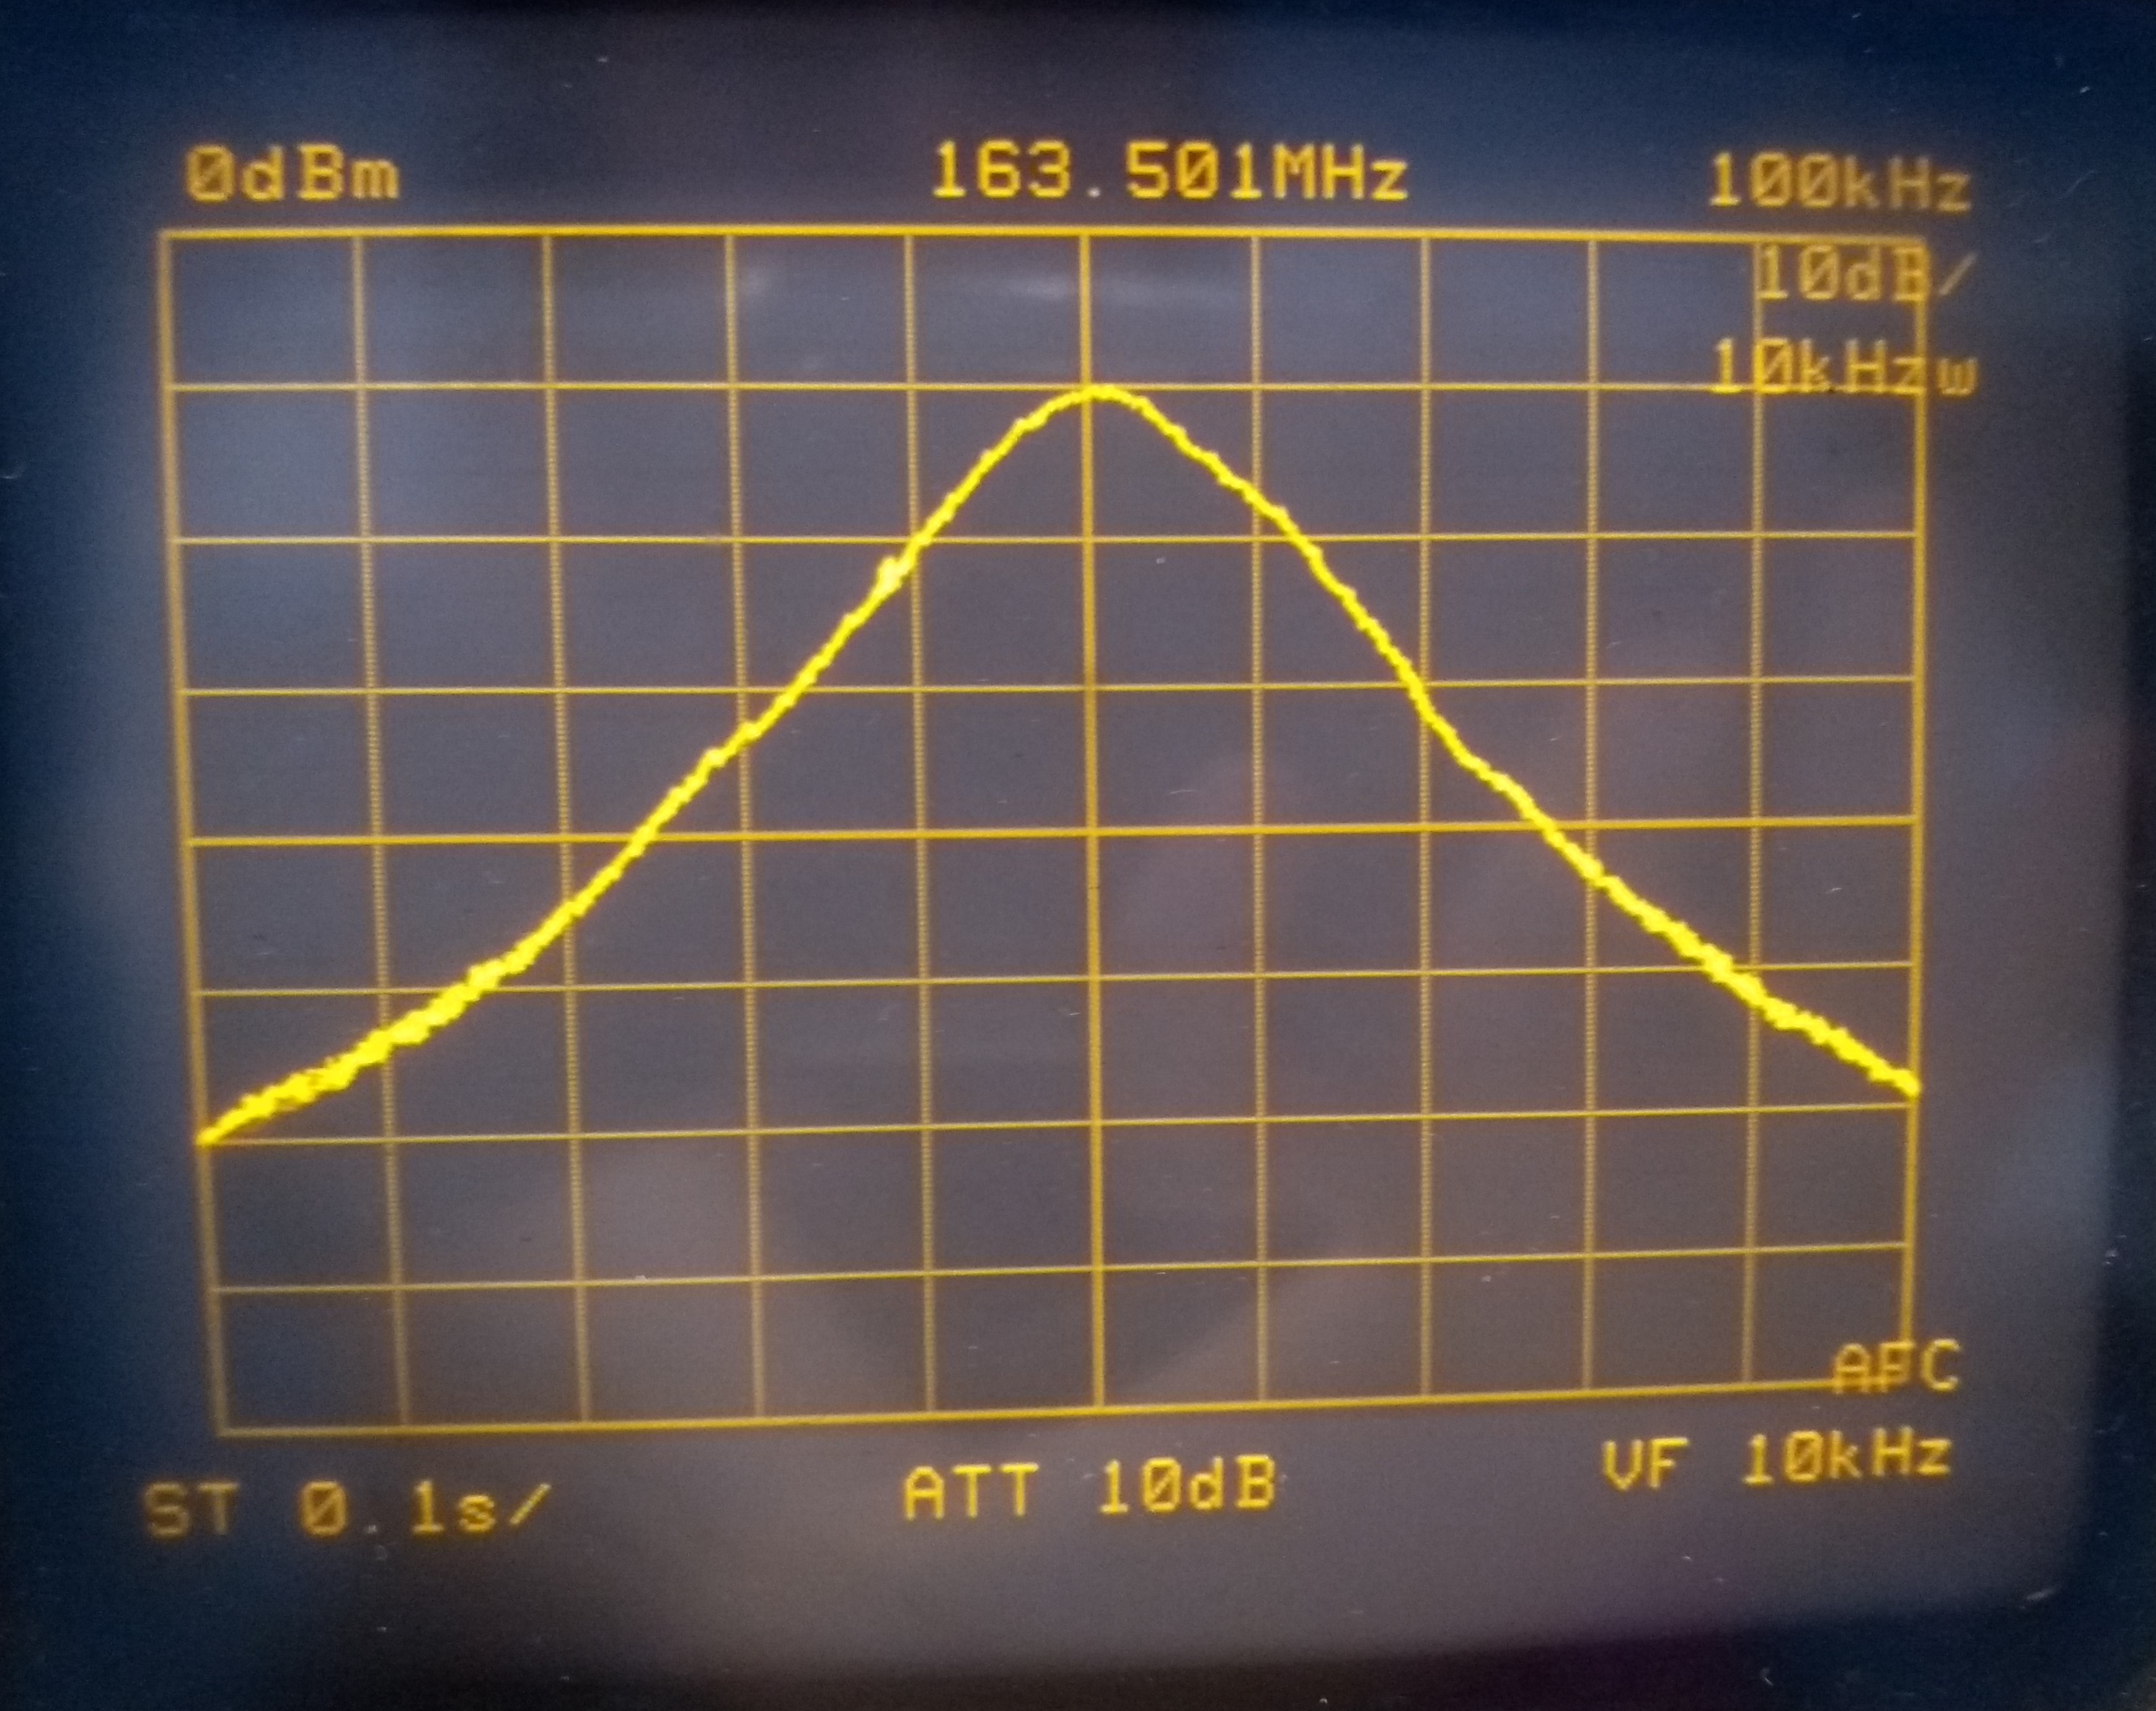
\includegraphics[scale=0.07]{imagenes/handy.jpg}}
	\caption{Espectro de la se\~nal generada por el \textit{handy}}
\end{figure}


\end{document}
